% ===================== 5. Results =====================
\section{Results}\label{sec:results}

\subsection{Main comparison}
Table~\ref{tab:main} reports the primary numbers; Figure~\ref{fig:results}
visualizes them. The wet-ink arm reaches $24.4\%$ ($11/45$) against the stock
baseline's $22.5\%$ ($18/80$)~--- a raw difference of $+1.9$ points with Wilson
intervals that overlap almost entirely. The frontier-only control scores $13.6\%$
($3/22$), which would suggest a dramatic $+10.8$-point editing effect; the paired
analysis shows this appearance is false.

\begin{table}[t]
\centering\small
\caption{GSM8K (first 45 indices), greedy decoding, LLaDA2.2-mini 4-bit NF4.
Baselines are from the paired v4 run (same model, quantization, prompts, indices).
NFE = network function evaluations per task.}\label{tab:main}
\begin{tabular*}{\textwidth}{@{\extracolsep{\fill}} l c c c c c}
\toprule
Arm & $n$ & Accuracy & Wilson 95\% CI & NFE & Rewrites/task \\
\midrule
\textbf{wetink\_w16} (ours, $W{=}16$) & 45 & \textbf{24.4\%} & $[14.2,\,38.7]$ & 206.6 & 6.9 \\
wetink\_noedit\_w16 (frontier only) & 22 & 13.6\% & $[4.7,\,33.3]$ & 201.1 & 0 \\
wetink\_w8 (narrow window)          & 10 & 20.0\% & $[5.7,\,51.0]$ & 202.7 & 5.6 \\
stock\_b32 (v4 baseline)            & 80 & 22.5\% & $[14.7,\,32.8]$ & 42.5  &~--- \\
noedit\_b32 (v4 baseline)           & 80 & 23.8\% & $[15.8,\,34.1]$ & 50.1  &~--- \\
\bottomrule
\end{tabular*}
\end{table}

\begin{figure}[t]
  \centering
  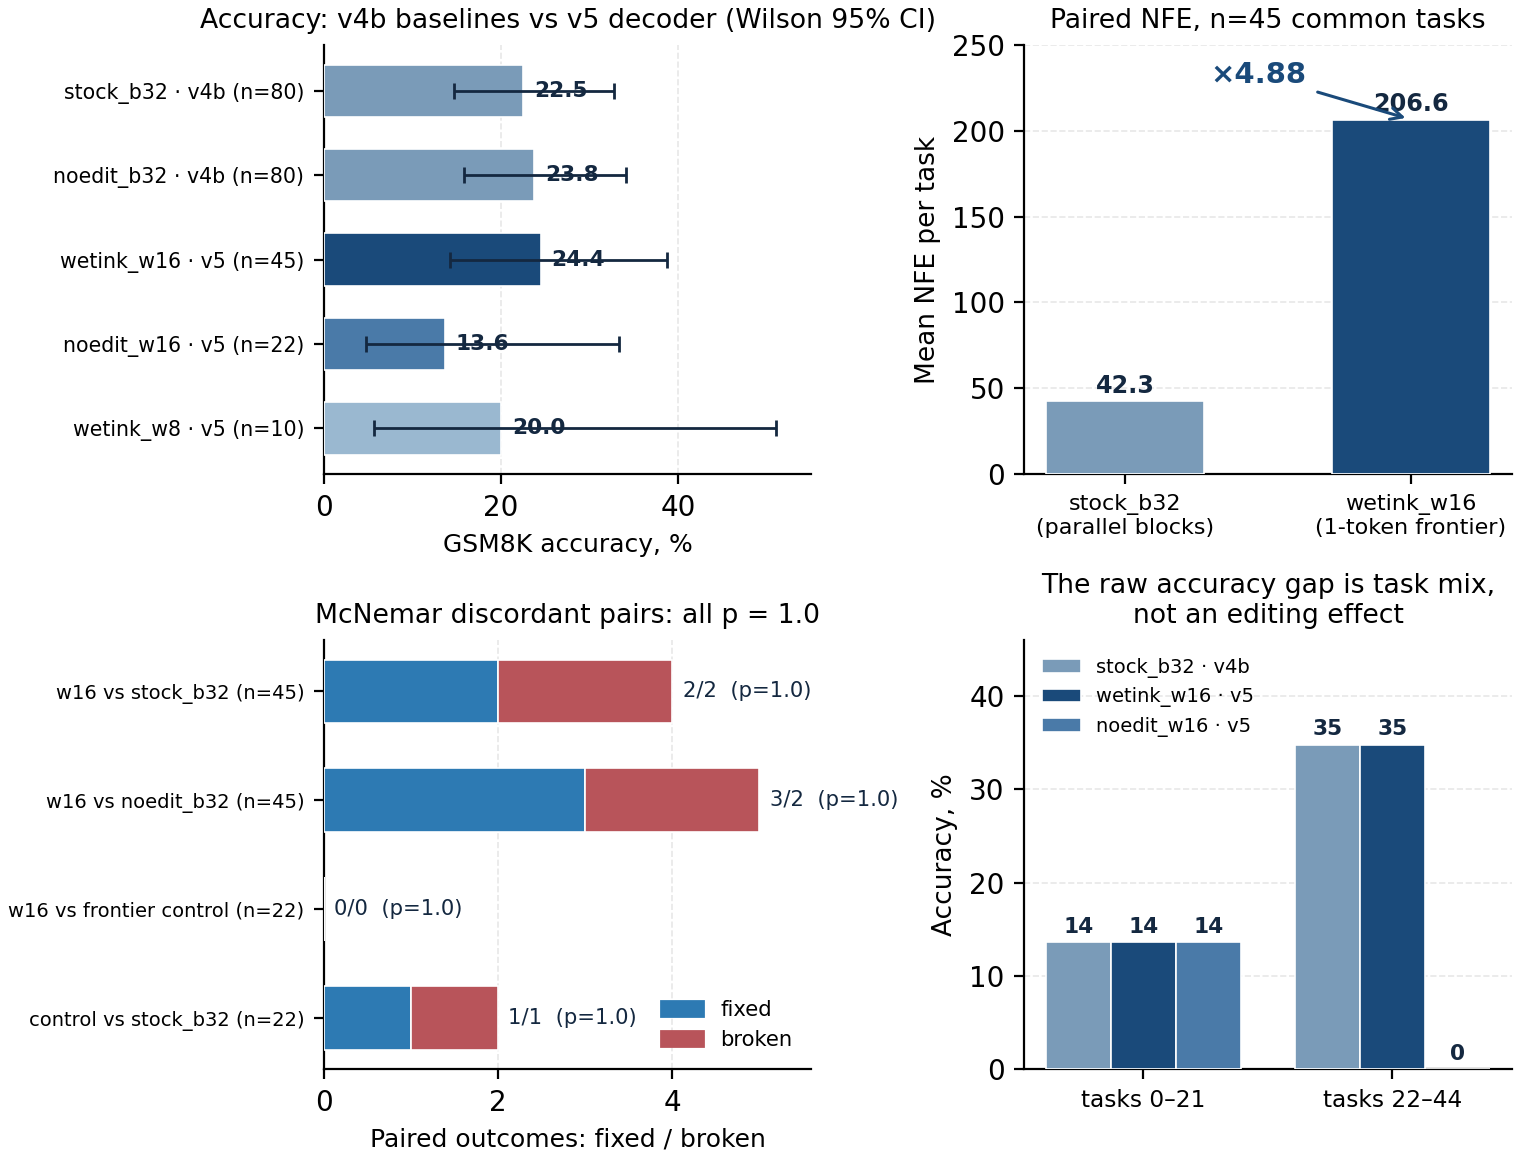
\includegraphics[width=0.96\textwidth]{fig_results.png}
  \caption{\textbf{Results.} (a) Accuracy with Wilson 95\% intervals for all arms.
  (b) Paired NFE on common tasks: stock versus wet-ink ($\times 4.88$). (c) McNemar
  discordant pairs for four comparisons~--- all $p{=}1.0$. (d) Segment analysis:
  on the hard tasks 0--21 every arm scores 13.6\%; the raw accuracy gap between
  arms reflects which segments they cover, not an editing effect.}
  \label{fig:results}
\end{figure}

\subsection{Paired exact analysis}
Table~\ref{tab:paired} gives the paired outcomes. Against the stock baseline, the
wet-ink arm solves exactly the same number of the 45 common tasks (11 versus 11),
with 2 outcomes fixed and 2 broken (exact McNemar $p{=}1.0$). Against the
frontier-only control on the 22 common tasks, the window edits flip \emph{zero}
outcomes ($3/22$ versus $3/22$, $0$ fixed, $0$ broken). The control itself matches
the stock baseline ($3/22$ versus $3/22$, $p{=}1.0$). In other words: the
one-token frontier costs nothing in accuracy relative to stock decoding, and the
editing window adds nothing on top of the frontier.

\begin{table}[t]
\centering\small
\caption{Paired exact McNemar on common task indices. `Fixed' = solved by the
second arm only; `broken' = solved by the first arm only.}\label{tab:paired}
\begin{tabular*}{\textwidth}{@{\extracolsep{\fill}} l c c c c c}
\toprule
Comparison (common $n$) & Score A & Score B & Fixed & Broken & $p$ \\
\midrule
wetink\_w16 vs stock\_b32 (45)    & 11/45 & 11/45 & 2 & 2 & 1.0 \\
wetink\_w16 vs noedit\_b32 (45)   & 11/45 & 10/45 & 3 & 2 & 1.0 \\
wetink\_w16 vs control (22)       & 3/22  & 3/22  & 0 & 0 & 1.0 \\
control vs stock\_b32 (22)        & 3/22  & 3/22  & 1 & 1 & 1.0 \\
\bottomrule
\end{tabular*}
\end{table}

\subsection{The task-composition artifact}\label{sec:artifact}
The $+10.8$-point raw gap between the wet-ink arm ($24.4\%$) and its own
frontier-only control ($13.6\%$) deserves a careful look, because it is exactly
the kind of number that is usually reported as a win. The mechanism is mundane:
the control arm exhausted its time budget after the first 22 tasks, and the first
22 GSM8K indices are systematically harder for this model~--- under 4-bit
quantization and a 160-token cap~--- than indices 22--44. On the hard segment
(tasks 0--21) \emph{every} arm scores exactly $13.6\%$: stock, control, and
wet-ink. On the easier segment the wet-ink arm scores $34.8\%$ and the stock
baseline $25.9\%$. The raw gap is therefore a statement about which tasks each
arm happened to cover, not about editing; the paired tests, which compare only
common indices, correctly report no effect. We flag this because unpaired
comparisons between unequally-truncated arms are easy to make in budget-limited
GPU settings and would have produced a false positive here.

\subsection{NFE accounting and mechanics}
The wet-ink arms cost $206.6$ NFE per task versus $42.3$ for stock on the same 45
tasks~--- a structural $\times 4.88$ multiplier, the price of committing one token
per forward pass. This multiplier is \emph{predictable} (it cannot churn: progress
is one mask per step by construction), unlike our v1 experience where a
training-free revision rule inflated NFE $9$--$13\times$ with
$\sim$589 re-masking events per block, $\sim$0.4 of which were real changes. In v5
the trained gate fires 6.9 real rewrites per task (churn 5.6)~--- the editing
machinery is demonstrably active, not disabled~--- and yet moves no outcomes.
Mechanics were verified on all 77 generations: bit-exact $W{=}0$ equivalence
(\texttt{ids\_equal=True}, NFE $97{=}97$), zero residual special tokens, and
deterministic outputs under $T{=}0$.

\subsection{Five versions as an ablation narrative}\label{sec:journey}
Table~\ref{tab:journey} summarizes the program that led here. Read as one
experiment, it is a five-step attack on the same hypothesis: \emph{can inference-time
token revision improve a fixed dLLM?} Training-free rules on the fixed Nemotron
model were harmful (v2--v3); the trained stock gate with a fixed block window is
neutral (v4); the trained gate with the sliding window it was arguably designed
for is still neutral (v5). Three independent, paired, consistently null results
--- in line with the calibration of \citet{remeval}~--- shift the burden of proof
toward approaches that change training, not decoding.

\begin{table}[t]
\centering\small
\caption{The five-version program. v1--v3 used
Nemotron-Labs-Diffusion-3B; v4--v5 use LLaDA2.2-mini. Paired statistics where
arm sizes permit.}\label{tab:journey}
\begin{tabularx}{\textwidth}{l l X}
\toprule
Ver. & Decoding scheme & Outcome (paired) \\
\midrule
v1 & confidence-gate re-masking each stock step & $+$6 pts GSM8K but
$\times 9$--$13$ NFE churn; termination invariant broken \\
v2 & full published revision cycles (RemeDi, CoDR) & termination restored;
RemeDi harmful at short blocks, CoDR near-neutral \\
v3 & full benchmark, $n{=}200$ GSM8K $+$ 164 HumanEval & RemeDi $-12.5$ to
$-31.5$ pts ($p{<}0.001$); CoDR neutral ($p{=}1.0$) \\
v4 & stock \texttt{generate()} parameter audit (12 arms, 403 gens.) & stock T2T
gate neutral ($p{=}1.0$), $-15\%$ NFE; window does not slide \\
v5 & \textbf{wet-ink: sliding window over trained gate} & \textbf{paired-identical
to stock ($p{=}1.0$) at $\times 4.88$ NFE} \\
\bottomrule
\end{tabularx}
\end{table}
